\begin{figure}[h!]
\centering

\begin{subfigure}[t]{0.48\textwidth}
\centering
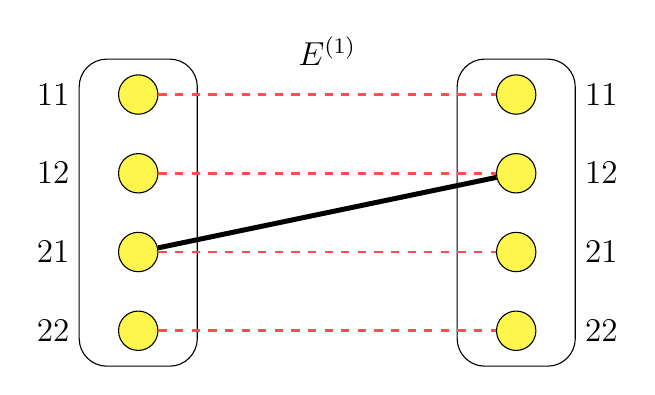
\begin{tikzpicture}[scale=1, every node/.style={font=\large}]
    % styles
    \tikzstyle{vtx}=[circle, draw=black, fill=yellow!70, minimum size=5mm, inner sep=0pt]
    \tikzstyle{dashededge}=[red!70, dashed, line width=1.0pt]
    \tikzstyle{solidedge}=[black, line width=1.8pt]

    % coordinates
    \def\lx{0}
    \def\rx{4.8}
    \def\yA{3}
    \def\yB{2}
    \def\yC{1}
    \def\yD{0}

    % enclosing boxes
    \draw[rounded corners=10pt] (-0.75,-0.45) rectangle (0.75,3.45);
    \draw[rounded corners=10pt] (4.05,-0.45) rectangle (5.55,3.45);

    % left vertices
    \node[vtx] (L11) at (\lx,\yA) {};
    \node[vtx] (L12) at (\lx,\yB) {};
    \node[vtx] (L21) at (\lx,\yC) {};
    \node[vtx] (L22) at (\lx,\yD) {};

    % right vertices
    \node[vtx] (R11) at (\rx,\yA) {};
    \node[vtx] (R12) at (\rx,\yB) {};
    \node[vtx] (R21) at (\rx,\yC) {};
    \node[vtx] (R22) at (\rx,\yD) {};

    % labels
   % labels: placed 0pt away from the enclosing boxes
    \node[anchor=east] at ([xshift=0pt]-0.75,\yA) {$11$};
    \node[anchor=east] at ([xshift=0pt]-0.75,\yB) {$12$};
    \node[anchor=east] at ([xshift=0pt]-0.75,\yC) {$21$};
    \node[anchor=east] at ([xshift=0pt]-0.75,\yD) {$22$};

    \node[anchor=west] at ([xshift=0pt]5.55,\yA) {$11$};
    \node[anchor=west] at ([xshift=0pt]5.55,\yB) {$12$};
    \node[anchor=west] at ([xshift=0pt]5.55,\yC) {$21$};
    \node[anchor=west] at ([xshift=0pt]5.55,\yD) {$22$};

    % title
    \node at (2.4,3.55) {$\mathbb{E}^{(1)}$};

    % dashed edges
    \draw[dashededge] (L11) -- (R11);
    \draw[dashededge] (L12) -- (R12);
    \draw[dashededge] (L21) -- (R21);
    \draw[dashededge] (L22) -- (R22);

    % solid edge
    \draw[solidedge] (L21) -- (R12);
\end{tikzpicture}
\caption{Adding any edge in $\bEE{1}$ bans the pairs in the identity permutation in the entire blueprint.}
\end{subfigure}
\hfill
\begin{subfigure}[t]{0.48\textwidth}
\centering
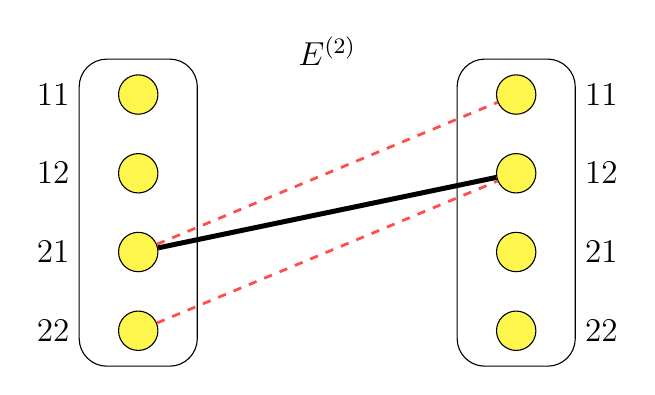
\begin{tikzpicture}[scale=1, every node/.style={font=\large}]
    % styles
    \tikzstyle{vtx}=[circle, draw=black, fill=yellow!70, minimum size=5mm, inner sep=0pt]
    \tikzstyle{dashededge}=[red!70, dashed, line width=1.0pt]
    \tikzstyle{solidedge}=[black, line width=1.8pt]

    % coordinates
    \def\lx{0}
    \def\rx{4.8}
    \def\yA{3}
    \def\yB{2}
    \def\yC{1}
    \def\yD{0}

    % enclosing boxes
    \draw[rounded corners=10pt] (-0.75,-0.45) rectangle (0.75,3.45);
    \draw[rounded corners=10pt] (4.05,-0.45) rectangle (5.55,3.45);

    % left vertices
    \node[vtx] (L11) at (\lx,\yA) {};
    \node[vtx] (L12) at (\lx,\yB) {};
    \node[vtx] (L21) at (\lx,\yC) {};
    \node[vtx] (L22) at (\lx,\yD) {};

    % right vertices
    \node[vtx] (R11) at (\rx,\yA) {};
    \node[vtx] (R12) at (\rx,\yB) {};
    \node[vtx] (R21) at (\rx,\yC) {};
    \node[vtx] (R22) at (\rx,\yD) {};

    % labels
   % labels: placed 0pt away from the enclosing boxes
    \node[anchor=east] at ([xshift=0pt]-0.75,\yA) {$11$};
    \node[anchor=east] at ([xshift=0pt]-0.75,\yB) {$12$};
    \node[anchor=east] at ([xshift=0pt]-0.75,\yC) {$21$};
    \node[anchor=east] at ([xshift=0pt]-0.75,\yD) {$22$};

    \node[anchor=west] at ([xshift=0pt]5.55,\yA) {$11$};
    \node[anchor=west] at ([xshift=0pt]5.55,\yB) {$12$};
    \node[anchor=west] at ([xshift=0pt]5.55,\yC) {$21$};
    \node[anchor=west] at ([xshift=0pt]5.55,\yD) {$22$};

    % title
    \node at (2.4,3.55) {$\mathbb{E}^{(2)}$};

    % dashed edges
    \draw[dashededge] (L21) -- (R11);
    \draw[dashededge] (L22) -- (R12);

    % solid edge
    \draw[solidedge] (L21) -- (R12);
\end{tikzpicture}
\caption{If the same edge was instead added to $\bEE{2}$, it would ban fewer but different pairs.}
\end{subfigure}

\caption{An illustration of ban constraints in a blueprint with $P=C=2$ with labels of vertices drawn next to them. Solid (black) edges show two possible edges in two different blueprints and dashed (red) edges show banned pairs resulting
from inclusion of each of these edges separately.}
\label{fig:ban}
\end{figure}